\chapter{Design Methodology}
\label{sec:design_methodology}

\section{Design Concept}

\subsection{Easy to Parameterize}

Hardware \gls{hwfra} implementation is designed to serve as a master node for multiple heterogeneous hardware DSA design to communicate like ROS concept. Each architecture design is also called node, \gls{dnn}  can to be parameterized to serve multiple heterogeneous nodes. This design is not re-configurable, that means, after the nodes are selected and the \gls{dnn}  is parameterized, it is fixed on he board and can’t change.
 
Not like traditional Operating System that managing resource like memory or hard disk, the major task for actionlib is to manage data communication, this architecture behave more like a network switch than hardware RTOS implementation like μC/OS. In order to make the design more flexible, the scheduler policy is designed to be configurable, but if a preempt able scheduler policy is chosen, it assumes that the servers must support interrupt management. Like AXIS Stream interface set, if the scheduler policy is fixed, it cannot be reconfigured on the run.


\subsection{Decouple switch from scheduler}
This architecture is designed for heterogeneous client and server nodes to connect. client nodes should be able to connect to any server nodes and vice versa. This architecture separate the switch topology from the scheduler policy by add a register between scheduler and switch. The scheduler can read and write the register and the switch can only read. 

The Atomic Client and Server Register hold the information for all nodes. For client nodes, it latches a bit signal indicating if the client is active and a unsigned integer for the server it connected to. For server nodes, the register hold a bit for active and a unsigned for it serving client.

The switch is a full combinational design.

\subsection{Decouple Scheduler Policy From the Scheduler Core}

Full connection for all clients and servers are expensive. We can save the resource usage by change the topology of the switch without affect other designs.

Therefore Scheduler communicate only with the priority table and don't care the topology of the switch component. Priority table can be written only by the scheduler and trigger the change of the atomic client server table before the next clock cycle arrives.


\subsection{3-level Preempting}

The \gls{dnn}  architecture is designed to connect every hardware architecture that communicate with AXIS Stream interface, \gls{dnn}  has been designed to be able to provides 3-level preemption support for preemptable hardware accelerators, \gls{dnn}  regard an architecture as OSLP if the this architecture support interrupt. Traditional RTOS is designed for microprocessors, which always contain a interrupt handling circuit, many large hardware instruction set architectures considered interrupt signal.  \gls{dnn}  also designed to be able to support RALP, which means the architecture follows the actionlib framework and implemented the callback interface of actionlib in hardware. 

% \section{Why No Goal List In Software Implementation}

% According to the concept of ROS Actionlib, this actionlib stored a goal list for a server to hold all coming goals from the subscribed ROS topic. But this 


\section{Module design}

This architecture is build for robotic system developers to transport robotic logic seamlessly to a full hardware design. It provides a structured communications layer above the hardware components of a heterogeneous compute cluster like the ROS software implementation did. Hardware ROS application developers need to implement robotic functions with an AXIS-Stream interface to communicate to each other. Then use parametrization tool to generate \gls{dnn}  I/O interface and connect the components together. Every component design is stand alone and heterogeneous so the development work can be easily distributed to multiple engineers and the design can be agilely reused without considering much about interface and synchronization.

This hardware architecture includes xilinx ip cores that synchronize clock rate and unified the AXIS-Stream form, therefore the architecture described following assumes a unified 8-bit wide AXIS-Stream transmission with tvalid, tready and tlast signals. This architecture also assumes a fixed ROS Actionlib signal set and a synchronized clock rate. This Actionlib signal set includes goal, cancel and finish for actionlib client nodes and accepted, rejected, aborted, preempted and succeed for server nodes.

\subsection{Hardware Architecture}

The center of this architecture is a switch. This switch read the information from the scheduler and change the connection of its inputs and outputs.

The I/O signals including AXIS Stream signals, actionlib control signals and actionlib states.

The switch is implemented fully combinational, therefore the re-connection will be done before next clock cycle. If a client or a server is not active, it will be connected to a all '0' dummy target.

 \begin{figure}[htb]
	\centering
	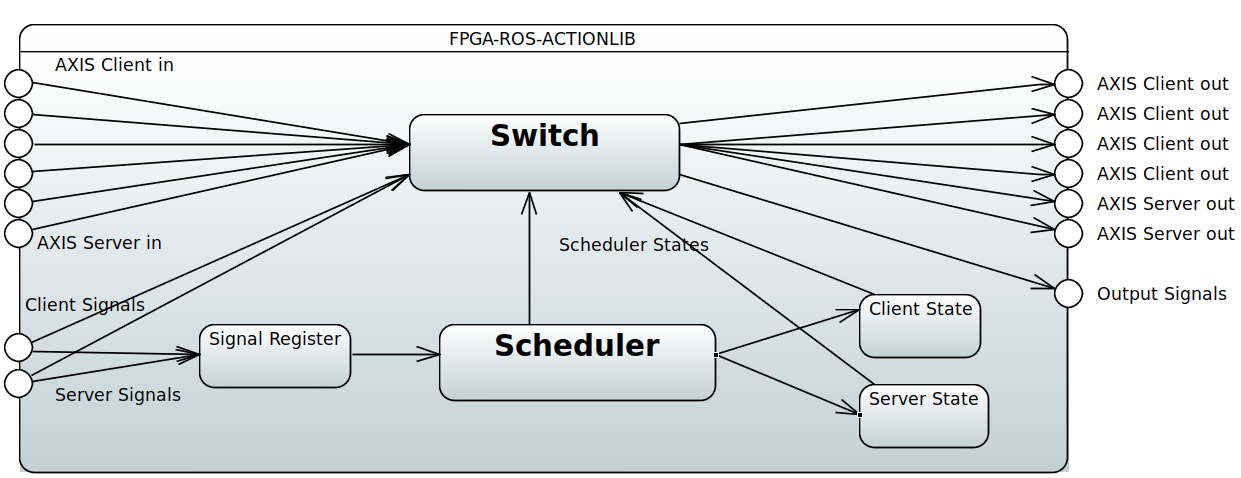
\includegraphics[width=.8\linewidth]{figures/fpac-tb.png}
	\caption{HWFRA-Component Design}
	\label{fig:hwfra-general}
\end{figure}

The scheduler has 3 parts, the center of the architecture lies priority table, a register that holds the priority numbers of all the clients. Only the scheduler core can modify the content and other parts read the register and make a change. The design of the scheduler core is therefore decoupled from other part of HWFRA and easy to change.



 \begin{figure}[htb]
	\centering
	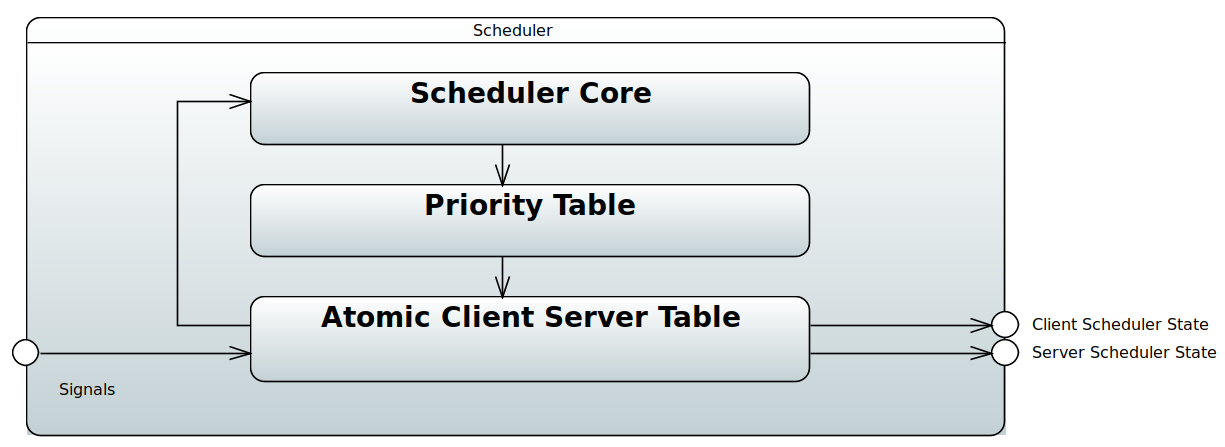
\includegraphics[width=.8\linewidth]{figures/fp-sc.png}
	\caption{Scheduler Design}
	\label{fig:hwfra-scheduler}
\end{figure}

This architecture lies completely in FPGA, it assumes the clients and servers can be anywhere in the system and communicate via AXIS Stream.


\begin{figure}[htb]
	\centering
	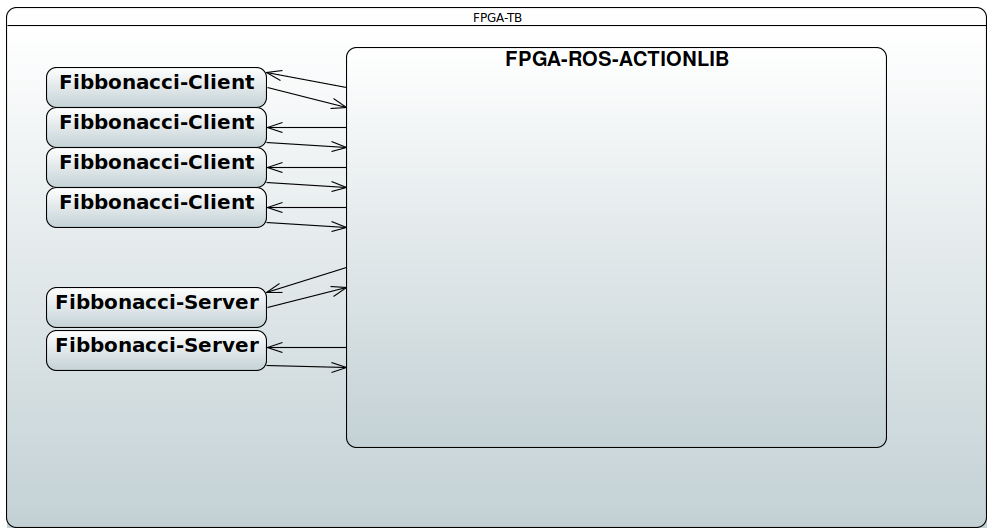
\includegraphics[width=.8\linewidth]{figures/fpga-tb.png}
	\caption{HWFRA in FPGA}
	\label{fig:hwfra-tb}
\end{figure}